\subsection{Manuelle Analog-zu-Digital-Wandlung} % (fold)
\label{sub:Manuelle_Analog-zu-Digital-Wandlung}
\begin{frame}
    \frametitle{Manuelle A/D Wandlung}
    \framesubtitle{}
     \begin{figure}[H]
     \begin{center}
             \includegraphics[scale=0.35]{./img/schaltung/manuelle_dac_0.png}
     \end{center}
     \end{figure}
\end{frame}
\begin{frame}
    \frametitle{Manuelle A/D Wandlung}
    \framesubtitle{}
    \begin{columns}[c]
        \column{0.5\textwidth}
            \begin{block}{}
                \begin{itemize}
                    \item Annährung der Referenzspannung durch digitale
                    Schaltung
                    \item LED and Komparator leuchtet solange digitales Signal
                    kleiner als Referenzspannung
                    \item Welcher Schaltvorgang ist am schnellsten?
                \end{itemize}
            \end{block}
        \column{0.5\textwidth}
             \begin{figure}[H]
             \begin{center}
                     \includegraphics[scale=0.2]{./img/schaltung/manuelle_dac_0.png}
             \end{center}
             \end{figure}
    \end{columns}
\end{frame}

\begin{frame}
    \frametitle{Verfahren}
    \framesubtitle{}
    \begin{block}{Approximationsverfahren}
        \begin{itemize}
            \item Zählverfahren: Binärzahl wird hochgezählt solange LED
            leuchtet
            \item Sukzessive Approximation: Beginnend beim MSB wird jeder
            Schalter getestet
        \end{itemize}
    \end{block}
\end{frame}

\begin{frame}
    \frametitle{Zählverfahren}
    \framesubtitle{}
    \begin{columns}[c]
        \column{0.4\textwidth}
            \begin{block}{}
                \begin{itemize}
                    \item Spannungswert wird langsam hochgezählt
                    \item im schlimmsten Fall: $2^n$ ($=255$) Schritte
                    \item Genauigkeit $\Delta U = \frac{1}{2}\frac{1}{256} V_{cc}$
                \end{itemize}
            \end{block}
        \column{0.6\textwidth}
            \begin{figure}[H]
            \begin{center}
                    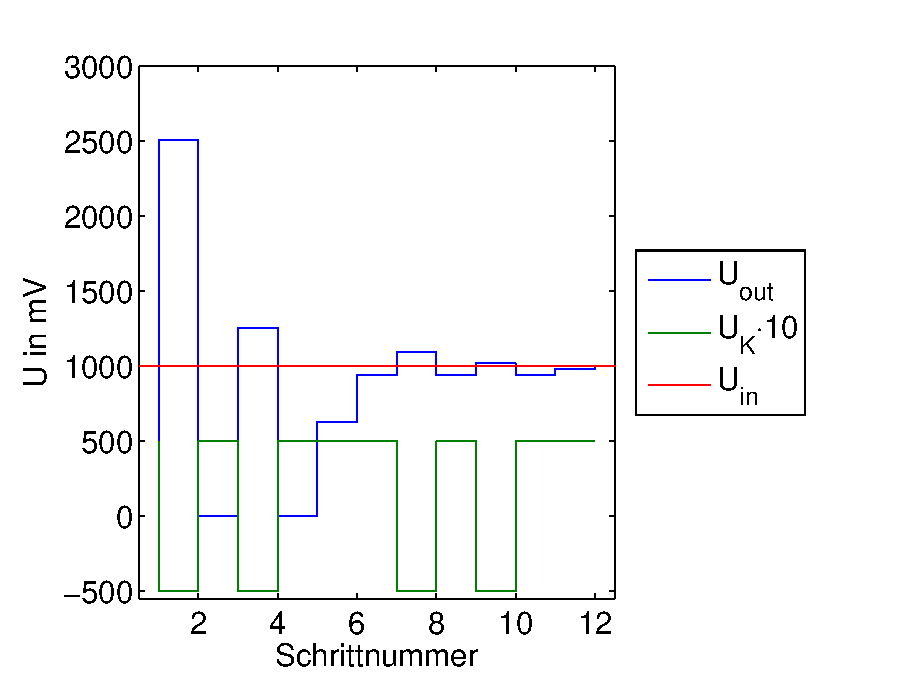
\includegraphics[scale=0.4]{./img/graph/Aufgabe2a2.eps}
            \end{center}
            \end{figure}
    \end{columns}
\end{frame}

\begin{frame}
    \frametitle{Sukzessive Approximation}
    \framesubtitle{}
    \begin{columns}[c]
        \column{0.4\textwidth}
            \begin{block}{}
                \begin{itemize}
                    \item Schaltung wird von MSB nach LSB getestet
                    \item Konstant $n$ ($=8$) Schritte
                    \item Genauigkeit $\Delta U = \frac{1}{2}\frac{1}{256} V_{cc}$
                \end{itemize}
            \end{block}
        \column{0.6\textwidth}
            \begin{figure}[H]
            \begin{center}
                    \includegraphics[scale=0.4]{./img/graph/Aufgabe2a.eps}
            \end{center}
            \end{figure}
    \end{columns}
\end{frame}

\begin{frame}
    \frametitle{Vergleich}
    \framesubtitle{}
    \begin{columns}[c]
        \column{0.6\textwidth}
            \begin{block}{Ergebnis}
                \begin{itemize}
                    \item Sukzessive Approximation sehr viel effizienter
                \end{itemize}
            \end{block}
            \begin{block}{Spannung zwischen $4.5V$ und $5V$}
                 \begin{itemize}
                     \item DAC kann die benötigte Spannung nicht aufbringen
                     \item Schaltung $S=0b11111111$ am Limit
                     \item $V_{cc},V_{ee}$ muss erhöht werden
                 \end{itemize}
            \end{block}
        \column{0.4\textwidth}
            \begin{figure}[H]
            \begin{center}
                    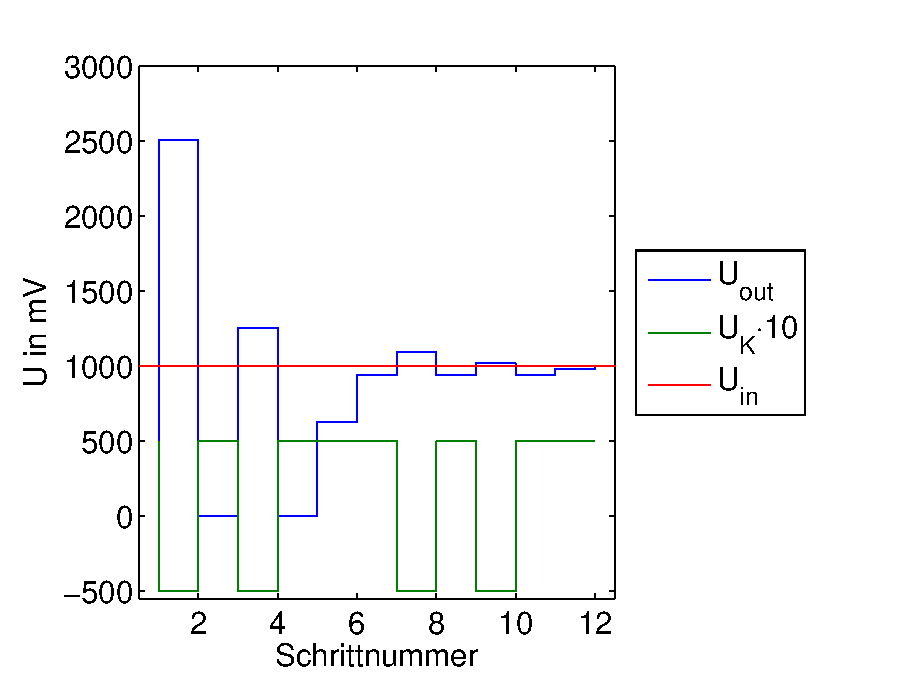
\includegraphics[scale=0.25]{./img/graph/Aufgabe2a2.eps}
            \end{center}
            \end{figure}
            \begin{figure}[H]
            \begin{center}
                    \includegraphics[scale=0.25]{./img/graph/Aufgabe2a.eps}
            \end{center}
            \end{figure}
    \end{columns}
\end{frame}

% subsection Manuelle Analog-zu-Digital-Wandlung (end)
